% Drawing 146/04-3 -- folder 146, batch 04, archive page 63 (PDF page 64).
% Transcription: En haut à gauche, un polyèdre en perspective formé de deux faces pentagonales (arêtes pleines et pointillées), les arêtes marquées $a, b, c, d, e$ et $a', b', c', d', e'$ ; une flèche courbe près de $b'$.
% Kind: polyhedron in perspective (two pentagonal faces). Method 2 (schematic redraw from the facsimile). Status: partial.
% Notes: Front pentagon (solid, edges a-e with a dot on each) and the second pentagon behind (dashed, edges a'-e'), the two long strokes through the right-hand vertices, the bold curved arrow by b'. The dashed back edges are scattered dashes; their joins are a reading, and the solid is not encoded: two pentagons with these joins do not determine a polyhedron unambiguously (prism? half a dodecahedron?). Label b'' / b' near the lower dashed vertex read as in the crop.
% Coordinates: 1 unit = 1 mm = 1/100 of the crop width (bbox in page fractions: [0.17, 0.12, 0.42, 0.27]).
% Redrawn by Claude (claude-opus-5-5), issue #73 pilot, 2026-11-07; not checked by a human; not compiled (no TeX in the session).
% Rights: reproduces part of the work -- behind RENDER_TRANSCRIPTS, never published by itself.
\documentclass[tikz,border=3pt]{standalone}
\usepackage{amsmath,amssymb}
\usetikzlibrary{patterns,arrows.meta}
\tikzset{pencil/.style={black!45}, struck/.style={black!35}, mark/.style={circle,draw,inner sep=1.3pt}, pt/.style={circle,fill,inner sep=0.9pt}, opt/.style={circle,draw,fill=white,inner sep=1.1pt}}
\begin{document}
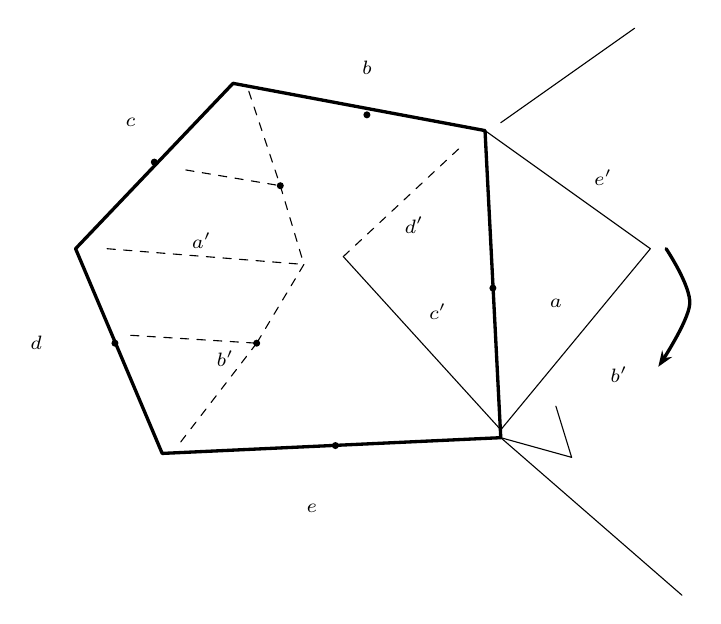
\begin{tikzpicture}[x=1mm,y=1mm,line cap=round,line join=round,font=\scriptsize]
\draw[very thick] (31,-17) -- (63,-23) -- (65,-62) -- (22,-64) -- (11,-38) -- cycle;
\node[pt] at (48,-21) {};
\node[pt] at (21,-27) {};
\node[pt] at (16,-50) {};
\node[pt] at (44,-63) {};
\node[pt] at (64,-43) {};
\draw (63,-23) -- (84,-38) -- (65,-61);
\draw (45,-39) -- (65,-61);
\draw[dashed] (45,-39) -- (60,-25);
\draw[dashed] (33,-18) -- (37,-30) -- (40,-40);
\draw[dashed] (25,-28) -- (37,-30);
\draw[dashed] (15,-38) -- (40,-40);
\draw[dashed] (40,-40) -- (34,-50);
\draw[dashed] (18,-49) -- (34,-50);
\draw[dashed] (34,-50) -- (24,-63);
\node[pt] at (37,-30) {};
\node[pt] at (34,-50) {};
\draw (65,-22) -- (82,-10);
\draw (65,-62) -- (88,-82);
\draw (65,-62) -- (74,-64.5) -- (72,-58);
\draw[very thick,-{Stealth[length=2mm]}] plot[smooth, tension=0.55] coordinates {(86,-38) (89,-45) (85,-53)};
\node[inner sep=1pt] at (48,-15) {\scriptsize $b$};
\node[inner sep=1pt] at (18,-22) {\scriptsize $c$};
\node[inner sep=1pt] at (6,-50) {\scriptsize $d$};
\node[inner sep=1pt] at (41,-71) {\scriptsize $e$};
\node[inner sep=1pt] at (72,-45) {\scriptsize $a$};
\node[inner sep=1pt] at (78,-29) {\scriptsize $e'$};
\node[inner sep=1pt] at (54,-35) {\scriptsize $d'$};
\node[inner sep=1pt] at (57,-46) {\scriptsize $c'$};
\node[inner sep=1pt] at (27,-37) {\scriptsize $a'$};
\node[inner sep=1pt] at (30,-52) {\scriptsize $b'$};
\node[inner sep=1pt] at (80,-54) {\scriptsize $b'$};
\end{tikzpicture}
\end{document}
